\begin{frame}[standout]
	Circular 3D Convolutions
\end{frame}

\begin{frame}{3D Circular Convolutions}
    \begin{center}
    	\includegraphics[width=0.75\textwidth,page=3]{convolutions_wpurple.pdf}	
    \end{center}

    \alert{Algorithm:} Forward $O(hwc \log hwc)$, Determinant $O(hwc)$
    \begin{algorithmic}[1]
  	  %\SetAlgoLined
		\REQUIRE{Image/activations $X\in\R^{h\times w \times c}$ and kernel $K\in\R^{h\times w\times c}$}.
		\STATE $X$ = DFT$_{3D}$($X$) 
		\STATE $K$ = DFT$_{3D}$($K$)
		\STATE $X$ = $X \odot  K$  
		\STATE $X$ = DFT$_{3D}^{-1}$($X$) 
	\end{algorithmic}
\end{frame}

\begin{frame}{Comparison with Periodic Convolutions}
	For $X, K \in \R^{h \times w \times c}$ and $W \in \R^{c \times c \times h \times w}$

	\alert{Circular 3D connvolutions}
	$$
		Z = F_{3D}^{-1}(F_{3D}(X) \odot F_{3D}(K))
	$$

	\alert{Periodic convolutions}
	$$
		z_{i} = F_{2D}^{-1}( \sum_{j=1}^c F_{2D}(W_{i, j}) \odot F_{2D}(X_{:,:,j})),
	$$

	\begin{center}
		\begin{tabular}{c|c c c c }
        	Type & Params & Forward & Inverse\\
    	\hline
        	Periodic & $h\cdot w \cdot c^2$ & $O(hwc^2)$ & $O(hwc^3)$ \\
        	3D-circular$^\dagger$ & $h \cdot w \cdot c^2$ & $O(hwc^2 \log (hwc))$ & $O(hwc^2 \log (hwc))$ \\
    	\end{tabular}
    \end{center}
	%\begin{tabular}{llll}
	%	\toprule
	%		Type &  Evaluation & Inversion & Log-determinant \\
	%	\midrule
	%	%1x1     &  $F_{1d}^{-1}\left[F_{1d}(x_{ij})\odot F_{1d}(k)\right]$ & $F_{1d}^{-1}(F_{1d}(x_{ij})\odot 1/F_{1d}(k))$  & $hw\sum_i \log (|F_{1d}(k)_i|$ \\
	%		3D      & $F^{-1}(F(X) \odot F(K))$ &  $F^{-1}(F(X) \odot 1/F(K))$  & $\sum_{ijk} \log(|F(K)_{ijk}|)$ \\
	%\end{tabular}
\end{frame}
